%!TEX root = ./Structure_rapport_final.tex


Resitue le sujet dans une problématique générale ;
 -restitue le sujet dans un cadre de gestion plus global
- doit également justifier le bien-fondé de l’étude en fonction des demandes
• Donne les objectifs qui ont été fixés pour répondre à la question posée ;
• Présente la démarche qui va permettre de répondre aux objectifs.


\subsection{Présentation des milieux marins profonds}
- communauté de poisson méso-bathy pélagiques 
- particuliarité des canyons 
- milieu peu connu, écosystème particulier --> communauté sur laquelle on travaille 
- Rôle de ces espèces dans les chaines trophiques (plus faibles maillons et MM/oiseaux)

Deep-sea is the largest marine habitat of Earth, and represents 95\% of ocean's volume \citep{danovaro2017,salazar2016}. From a biology perspective, deep-sea encompasses everything underneath euphotic (or epipelagial) zone, where the solar radiations are too low and precludes photosynthesis \citep{danovaro2017,salazar2016} (see Figure~\ref{fig:dsl}). Between 200 to 1000m deep (mesopelagic zone), light fades and temperature decreases, because solar luminance is absorbed exponentially in upper sea layers \citep{reynolds2001}. After 1000m deep (bathypelagic zone), no sunlight remains and the habitat is pitch-black; temperature is stable, between -1.8 to 2°C and pressure increases from 20 to more than 1100 atm. 
Despite these extremes conditions, deep-sea is far from being lifeless. In fact, deep-sea is considered to be the largest biome of the Earth, and contains 70\% of ocean's microbial cells and 60\% of its heterotrophic activity \citep{salazar2016}. 

\begin{figure} [!htbp]
	\begin{center}
		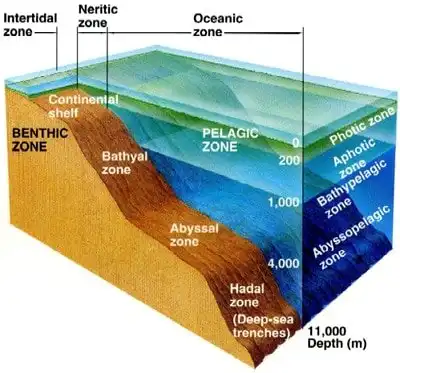
\includegraphics[width=0.8\textwidth]{sea_layers.png}
	\end{center}
	\caption[Petite légende]{Sea layers along depth, from \citep{fig_deep_sea}}
	\label{fig:dsl}
\end{figure}



\subsection{Axes pour une meilleure connaissance de ces écosystèmes}
- comment les espèces se partagent les ressources (bcp d'études déjà terrestres)
         --> focus sur cette communauté particulière qui est pour l'instant peu connue

- 2 approches possibles: 
		- espèce-centrée : seule ou en compétition --> mais limitant pour la comparaison entre écosystèmes différents. 
		- communautaire : certaines espèces sont-elles redondantes ? Plusieurs espèces
occupent la même niche en cas de chevauchement, occupent la même niche fonctionnelle. Se focaliser
sur les fonctions plutôt que sur l'espèce. --> Permet une généralisation de la méthode et une comparaison entre écosystèmes
		- Individus appartenant à la meme niche peuvent être considérés comme appartenant
à la même boîte fonctionelle. 
==> Caractériser un écosystème par les fonctions qu'ils présentent plutôt que par ses espèces

\subsection{Présentation de la démarche et des objectifs}
- mieux connaitre ces communautés à travers les niches qu'elles occupent dans les écosystèmes
- caractériser leurs niches trophiques, comportements, habitats, sensibilité des espèces, 
particularité des espèces, voir les avantages de partager les niches 
- Envisager une approche universelle, permettant la comparaison d'écosystèmes

- Hypothèses: chevauchement de niches entre les espèces, entrainant de la compétition entre les espèces ayant des fonctions similaires, ou ségrégation, où les espèces
utilisent des ressources distinctes et ont des fonctions différentes

